% !TEX root = ../../../main.tex
% 来源：中学数学实验教材·第三册（高中数学）
% 章节：任意角的三角函数 / 任意角的三角函数
% 原始文件：6.tex，行 1108-1140
% 类型：tikz
% ---
\begin{tikzpicture}[>=latex, scale=1.5]
\begin{scope}
 \draw[->] (-1.5,0)--(1.5,0)node[right]{$x$};
 \draw[->] (0,-1.5)--(0,1.5) node[right]{$y$};
\draw[->, thick] (0,0)--(30:1)node[right]{$P\left(\tfrac{\sqrt{3}}{2},\tfrac{1}{2}\right)$};
\draw(30:1)--(1.732/2,0);
\node at (-.2,-.2){$O$};
\draw (0,0) circle(1);
\draw[->] (.5,0) arc (0:30:.5)node[right]{$\tfrac{\pi}{6}$};
\end{scope}

\begin{scope}[xshift=4cm]
    \draw[->] (-1.5,0)--(1.5,0)node[right]{$x$};
    \draw[->] (0,-1.5)--(0,1.5) node[right]{$y$};
   \draw[->, thick] (0,0)--(45:1)node[right]{$P\left(\tfrac{\sqrt{2}}{2},\tfrac{\sqrt{2}}{2}\right)$};
   \draw(45:1)--(1.414/2,0);
   \node at (-.2,-.2){$O$};
   \draw (0,0) circle(1);
   \draw[->] (.35,0) arc (0:45:.35)node[right]{$\tfrac{\pi}{4}$};
   \end{scope}


\begin{scope}[xshift=2cm, yshift=-2.5cm]
    \draw[->] (-1.5,0)--(1.5,0)node[right]{$x$};
    \draw[->] (0,-1.5)--(0,1.5) node[right]{$y$};
   \draw[->, thick] (0,0)--(60:1)node[right]{$P\left(\tfrac{1}{2},\tfrac{\sqrt{3}}{2}\right)$};
   \draw(60:1)--(.5,0);
   \node at (-.2,-.2){$O$};
   \draw (0,0) circle(1);
   \draw[->] (.35,0) arc (0:60:.35)node[right]{$\tfrac{\pi}{3}$};
   \end{scope}

\end{tikzpicture}
